%%%%%%%%%%%%%%%%%%%%%%%%%%%%%%%%%%%%%%%%%%%%%%%%%%%%%%%%%%%%%%%%%%%%%%%%%%%%%%%%
% Chapter 2: Conceptos
%%%%%%%%%%%%%%%%%%%%%%%%%%%%%%%%%%%%%%%%%%%%%%%%%%%%%%%%%%%%%%%%%%%%%%%%%%%%%%%%

%++++++++++++++++++++++++++++++++++++++++++++++++++++++++++++++++++++++++++++++
% \section{Visión estéreo}
% \label{2:sec:2}
% http://vision.deis.unibo.it/~smatt/Seminars/StereoVision.pdf
% http://www.cesfelipesegundo.com/revista/articulos2011/Guerrero,%20J.M.pdf

La visión estereoscópica o visión estéreo, es la técnica capaz de extraer
información tridimensional (profundidad) a partir de la posición relativa de un
objeto en imágenes bidimensionales al ser observado desde distintos ángulo por
dos o más cámaras separadas a una cierta distancia.

%--------------------------------------
\subsection{Calibración}

%--------------------------------------
\subsection{Adquisición}

Usando dos cámaras, el procedimiento a seguir para la adquisición del entorno
es capturar dos imágenes de una misma escena, desde dos cámaras separadas
ligeramente. De esta forma, las imágenes obtenidas, también tendrán un pequeño 
desplazamiento entre sí.

De manera más formal, se obtiene que para cada imagen capturada por las
cámaras, un objeto está en puntos diferentes del plano. Esta triangulazión
entre el punto P y Q y el origen de referencia, provocan una sensación de
profundidad. Mediante el sistema tradicional de una sola cámara, este punto
estaría en las mismas coordenadas.

\begin{figure}[!th]
  \begin{center}
    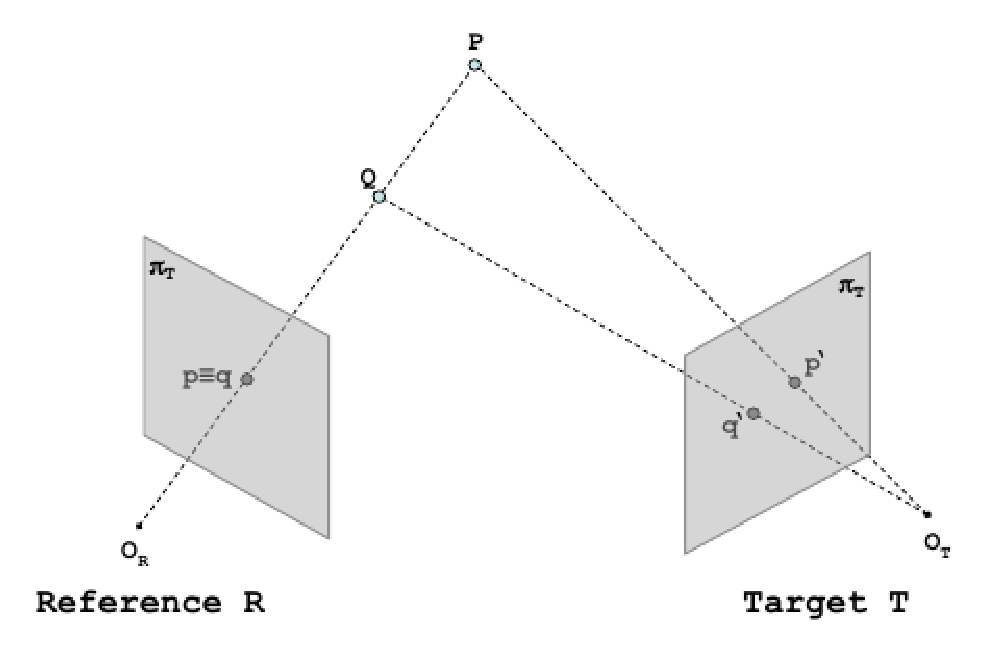
\includegraphics[width=0.7\textwidth]{images/cap2/VisionEstereo.eps}
    \caption{Diferencias entre una y dos cámaras}
    \label{fig:VisionEstereo}
  \end{center}
\end{figure}

Con estos datos, se pueden poner en correspondencia cada punto de ambas
imágenes, para obtener una imagen de disparidad (más información en la sección 
2.2.4).

%--------------------------------------
\subsection{Geometría de las cámaras}
% https://en.wikipedia.org/wiki/Parallax
% http://www.cesfelipesegundo.com/revista/articulos2011/Guerrero,%20J.M.pdf
En función de la posición relativa de las cámaras entre sí, se pueden apreciar
dos métodos principales:

\begin{itemize}
  \item \textbf{Visión paralela:} las cámaras están paralelas entre sí y están
  separadas por una línea horizonal (línea base). El objetivo que visualiza
  cada cámara es perpendicular respecto a la línea base, mientras que las
  líneas de correspondencia que unen los puntos de una imagen respecto a la
  otra son horizontales.

  \begin{minipage}{\linewidth}
      \centering
      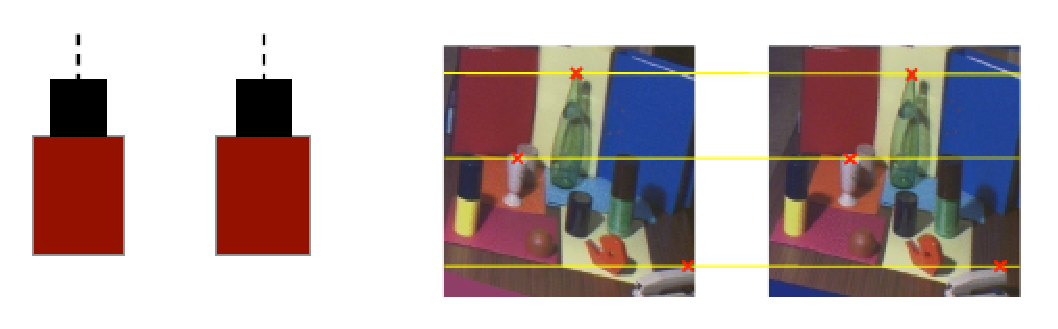
\includegraphics[width=0.7\textwidth]{images/cap2/VisionParalela.eps}
      \captionof{figure}{Visión paralela}
      \label{fig:VisionParalela}
  \end{minipage}

  \item \textbf{Visión cruzada:} las cámaras no están paralelas entre sí,
  tienen una inclinación de tal forma que el objetivo de cada cámara apunta
  hacia el lado contrario de una imagen. Por lo que los ejes ópticos se cruzan
  entre sí. Las líneas de correspondencia, también tienen sufren una
  inclinación.

  \begin{minipage}{\linewidth}
      \centering
      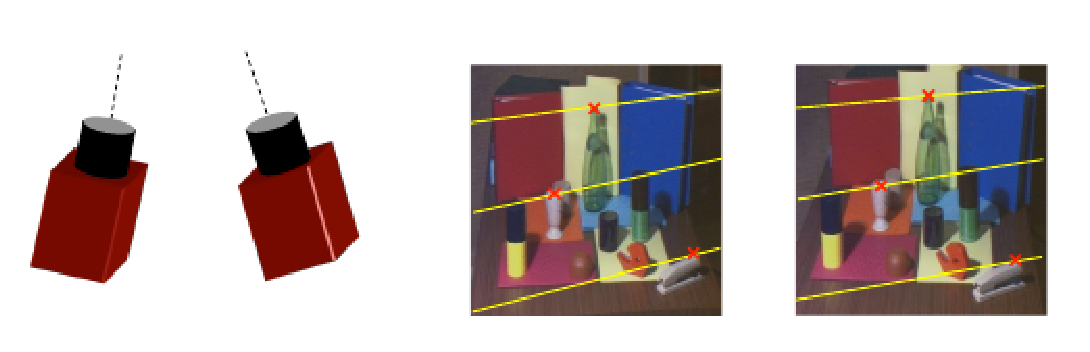
\includegraphics[width=0.7\textwidth]{images/cap2/VisionCruzada.eps}
      \captionof{figure}{Visión cruzada}
      \label{fig:VisionCruzada}
  \end{minipage}
\end{itemize}

% http://vfxio.com/PDFs/Parallel_vs_Converged.pdf
La visión cruzada tiene la desventaja de distorsionar las imágenes capturadas.
En la figura 2.4 se puede observar este efecto al fotografíar un muro de
ladrillos. Sin embargo, dependiendo del tipo de escena que se capture, esta
distorsión puede suponer un problema o no.

\begin{figure}[!th]
  \begin{center}
    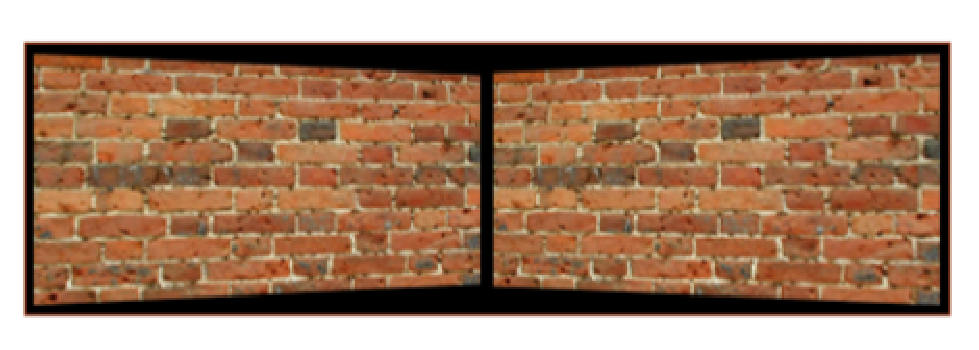
\includegraphics[width=0.5\textwidth]{images/cap2/VisionCruzadaMuro.eps}
    \caption{Muro distorsionado por visión cruzada}
    \label{fig:VisionCruzadaMuro}
  \end{center}
\end{figure}

La visión paralela por su parte, no distorsiona las imágenes capturadas, pero
también cuenta con otra serie de problemas. A pesar de ello, la visión paralela
suele ser la más utilizada para la visión estéreo.

%--------------------------------------
\subsection{Rectificación}
% https://en.wikipedia.org/wiki/Image_rectification

%--------------------------------------
\subsection{Disparidad}
% http://es.slideshare.net/RicardoSnchezCastill/vision-artificial-49264591
% http://stackoverflow.com/questions/17607312/difference-between-disparity-map-and-disparity-image-in-stereo-matching
% http://iie.fing.edu.uy/publicaciones/2005/Lec05a/Lec05a.pdf
La disparidad de dos imágenes establece la correspondencia entre los píxeles o
características que existen entre ambas para obtener la profundidad de la
escena.

El objetivo final es poder construir una \textbf{imagen o mapa de disparidad}.

\begin{figure}[!th]
  \begin{center}
    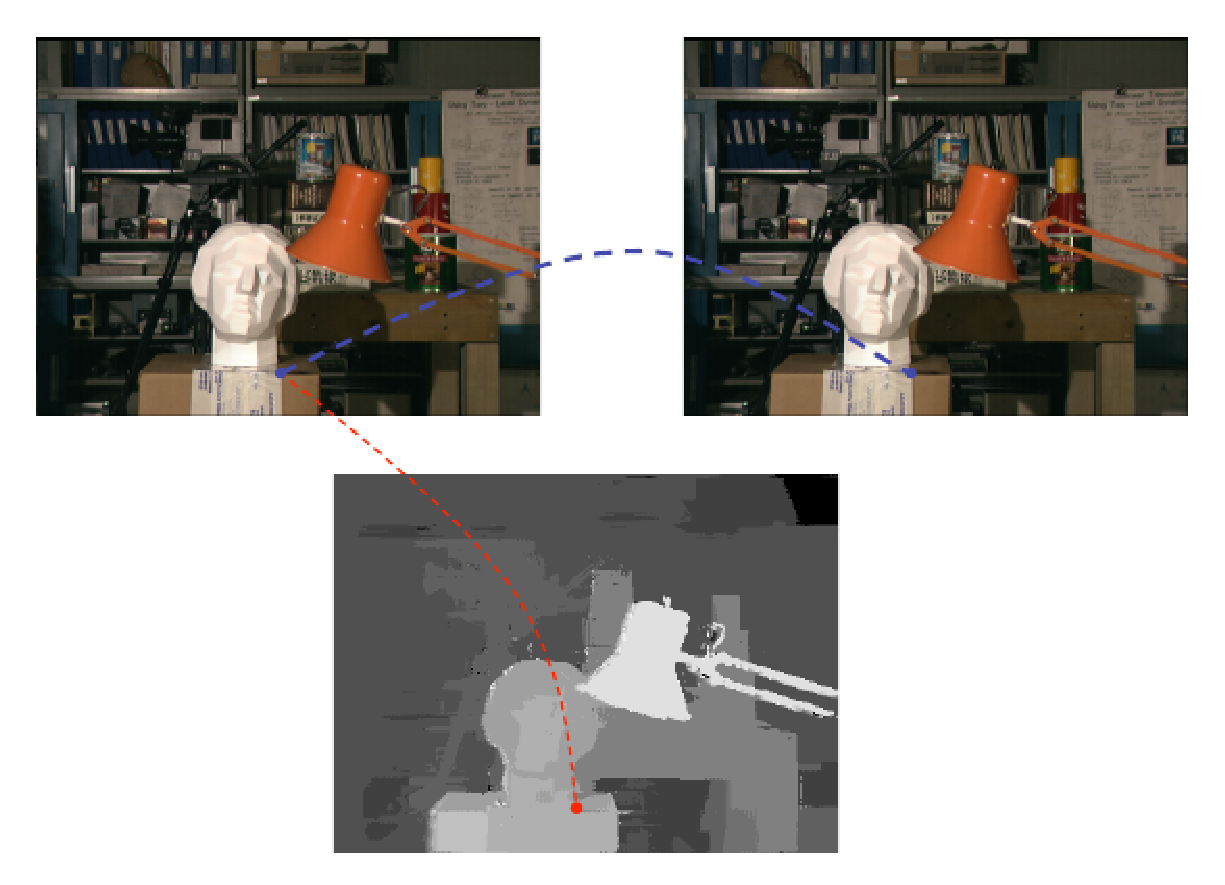
\includegraphics[width=0.7\textwidth]{images/cap2/MapaDisparidad.eps}
    \caption{Mapa de disparidad a partir de imágenes en estéreo}
    \label{fig:MapaDisparidad}
  \end{center}
\end{figure}







% Disparidad....

% http://www.cesfelipesegundo.com/revista/articulos2011/Guerrero,%20J.M.pdf
% http://dmi.uib.es/~abasolo/cursorealidad/paco/Estereoscopia.html


%--------------------------------------
\subsection{Reconstrucción 3D}

%--------------------------------------
\subsection{Aplicaciones}
% https://www.ptgrey.com/tan/10570
La visión artificial resulta de gran utilidad en diferentes áreas de
aplicación, tanto en acciones repetitivas como peligrosas:


\begin{itemize}
  \item \textbf{Inspección y ensamblaje industrial:} el proyecto "Randon Bin
  Picking" (RBP) hace uso de visión estéreo para la búsqueda de piezas entre
  objetos de todo tipo para su rápida recuperación.
  % http://www.worldscientific.com/doi/suppl/10.1142/8766/suppl_file/8766_chap01.pdf
  \item \textbf{Apoyo en el diagnóstico médico:} en las últimas décadas la
  visión artificial se ha hecho un importante en la medicina para detectar,
  analizar y reconstruir la información obtenida.
  % http://www.ri.cmu.edu/pub_files/pub4/matthies_larry_2007_1/matthies_larry_2007_1.pdf
  \item \textbf{Exploración espacial:} en el proyecto de exploración Mars Rover
  (Mars Exploration Rover Mission) tiene como objetivo explorar la superficie
  de Marte en busca de rocas u otros elementos que prueben la existencia de
  agua.
  \item \textbf{Seguimiento (Tracking):} se hace uso en innumerables
  situaciones de carácter estadístico como contar el número o de en áreas de
  vigilancia y seguridad monitorizando trayectorias.
\end{itemize}

%++++++++++++++++++++++++++++++++++++++++++++++++++++++++++++++++++++++++++++++
